\chapter{Adapter Pattern}

%\includegraphics[width=0.5\columnwidth]{imagefile}

\section{Định nghĩa}
Adapter Pattern chuyển đổi giao diện của một lớp thành giao diện khác mà client mong muốn. Adapter cho phép các lớp hoạt động cùng nhau mà thông thường đó là không thể vì các giao diện không tương thích.

\section{Mục đích sử dụng}
Trong thực tế có những tình huống khi muốn sử dụng một loại dữ liệu hay thư viện mà API của nó không tương thích với API mà mình đang sử dụng. Khi đó chúng ta không muốn thay đổi hay chỉnh sửa code/hệ thống của nhà cung cấp và của mình vì những thay đổi đó có thể chỉ là nhất thời, trong tương lai có thể không sử dụng đến API của nhà cung cấp nữa. Vì thế, Adapter Pattern được sử dụng để chuyển đổi giao diện(interface) của một lớp thành giao diện khác mà client mong muốn.

\section{Mô hình cấu trúc}
\begin{center}
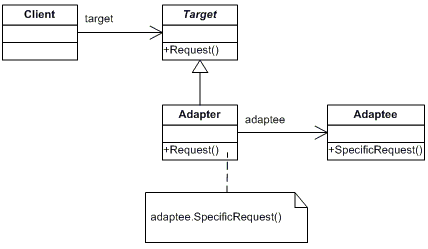
\includegraphics{GALLEYS/images/chapter6/diagram}\\
\end{center}
Các thành phần:
\begin{itemize}
\item Client làm việc trực tiếp qua Target interface.
\item Adapter sẽ implement Target interface đó.
\item Adapter dịch yêu cầu của client thành những yêu cầu cụ thể mà adaptee hiểu.
\item Adaptee (tạm gọi là class thích ứng, có nhiệm vụ thích ứng với client) là class sẽ đáp ứng yêu cầu của client nhưng hiểu theo cách mà adapter truyền lại. Những class này thường chứa những dịch vụ hữu dụng mà nhiều class khác cần dùng tới, thường là những legacy class (những class ở phiên bản trước, được thay thế thành class phiên bản cao cấp hơn), những class bên thứ ba hoặc có nhiều dependencies.
\end{itemize}
Các bước triển khai:
\begin{enumerate}
\item Client gửi yêu cầu ở interface.
\item Tạo một lớp adapter để triển khai client interface đó.
\item Lớp adapter giữ reference (tham chiếu) đến adaptee (cách phổ biến là truyền nó vào tham số của constructor (hàm dựng) của adapter).
\item Adapter lần lượt triển khai các methods (phương thức) của client interface, làm những công việc như chuyển đổi dữ liệu trước khi điều hướng các trách nhiệm cho lớp adaptee thực sự xử lý.
\item Client nhận được kết quả họ muốn và không biết có một adapter ở giữa gắn kết 2 bên. Ta có thể thay đổi hoặc mở rộng adapter mà không ảnh hưởng đến code của client.
\end{enumerate}
Ta xét một ví dụ cụ thể sau: Nếu có một con vật nào đó đi lại như một con vịt và kêu như một con vịt, như vậy nó sẽ là một con vịt! Hoặc... nó cũng có thể là một con gà tây với một adapter của con vịt!
Trước hết, ta có một mô hình mô phỏng một con vịt có hơi khác một chút (nó sẽ có hai khả năng là kêu và bay – tất nhiên sẽ có kiểu kêu và bay đặc trưng):\\
\begin{center}
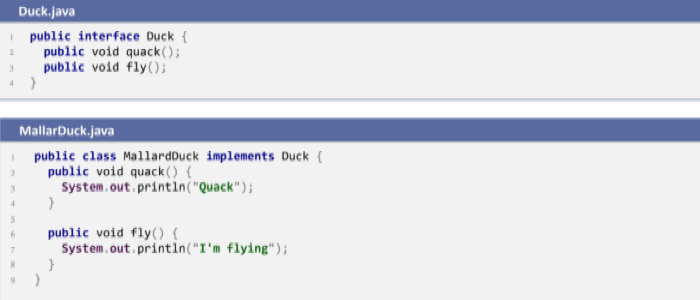
\includegraphics{GALLEYS/images/chapter6/code1}\\
\end{center}
Có một kẻ gian xảo nào đấy muốn xâm nhập vào quá trình mô phỏng này. Nó có kiểu kêu, kiểu bay không hề giống một con vịt:
\begin{center}
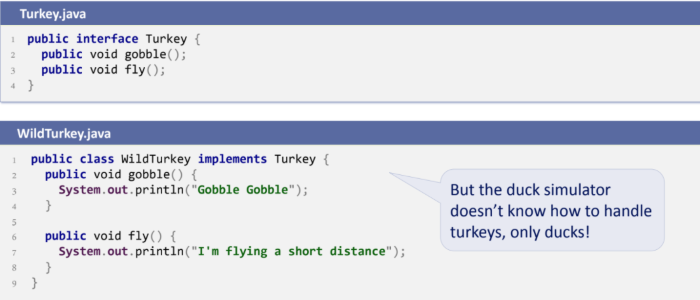
\includegraphics{GALLEYS/images/chapter6/code2}\\
\end{center}
Rõ ràng trình mô phỏng một con vịt sẽ không biết xử lý những con gà tây (Turkey) này như thế nào, chỉ có thể xử lý được những con vịt. Và giải pháp ở đây sẽ là... viết một adapter mà làm cho một con gà tây trông giống một con vịt:
\begin{center}
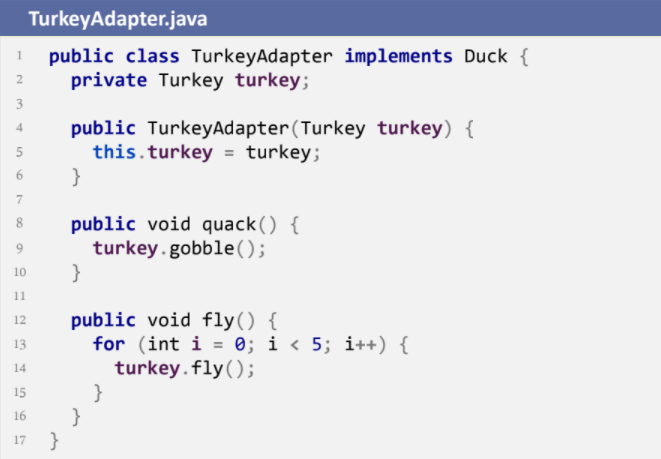
\includegraphics{GALLEYS/images/chapter6/code3}
\end{center}
Chúng ta tiến hành theo các bước như sau:
\begin{enumerate}
\item Adapter Turkey implements (thừa kế) giao diện mục tiêu (Duck) để có “hình hài” của con vịt - Duck (trong mối quan hệ is-a, hay nói cách khác đó là việc adapter tương thích dữ liệu với Duck) và nó sẽ thể hiện hành vi của con gà tây (Turkey). Tức là API giống của vịt nhưng kết quả là tiếng kêu của con gà tây.
\item Adaptee (Turkey) được chuyển qua hàm dựng và được lưu trữ nội bộ.
\item Các yêu cầu bằng code của client được ủy quyền (kỹ thuật deligation) cho các phương thức tương ứng trong adaptee (ở đây là để thực hiện hành vi của con gà tây).
\item Adapter là một lớp chính thức, có thể chứa các biến bổ sung và các phương thức để hoàn thành công việc của mình; có thể sử dụng đa hình như một con vịt (Duck). Để sử dụng hành vi/phương thức riêng của adapter thì phải tiến hành downcast để về dữ liệu thật (Duck -> adapter). Tóm lại, adapter chỉ đơn giản là để “chuyển” từ con gà tây sang con vịt.
\end{enumerate}
\begin{center}
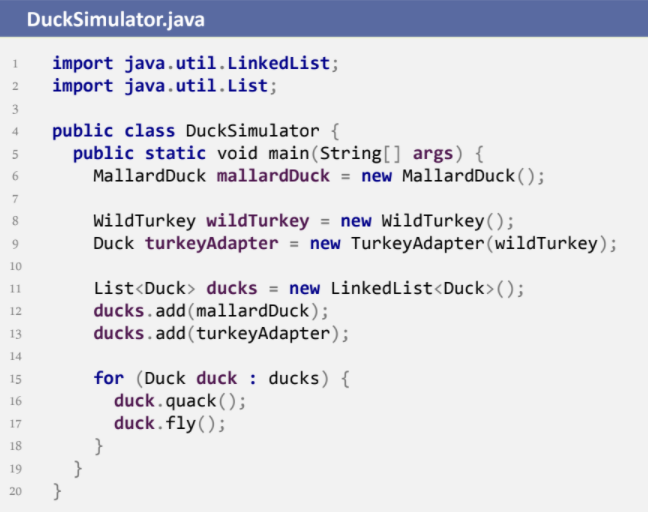
\includegraphics{GALLEYS/images/chapter6/code4}
\end{center}

\section{Adapter Pattern trong thực tế}
Adapter được ứng dụng rộng rãi trong nhiều trường hợp, ta thường thấy Adapter xuất hiện trong những tình huống cần nâng cấp hệ thống cũ và có nhiều class cũ nhưng vẫn chứa phương thức quan trọng, làm cho hệ thống hiệu quả hơn thông qua việc làm cho các component giao tiếp với nhau dù không liên quan đến nhau. Một ví dụ thực tiễn: Sử dụng Enumerator như một Iterator trong Java:\\
\begin{center}
	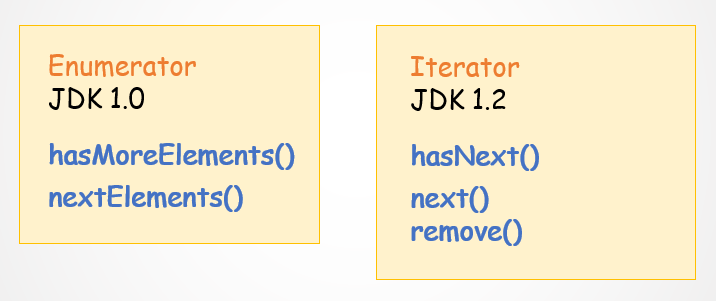
\includegraphics{GALLEYS/images/chapter6/example1}\\
\end{center}

Ở Java, Enumerator và Iterator đều là những con trỏ để duyệt và truy cập phần tử của một collection như Vector, Stack, Hashtable,... Enumerator xuất hiện ở JDK 1.0 và Iterator được ra mắt ở JDK 1.2. Enumerator cung cấp 2 phương thức hasMoreElement() và nextElement() để kiểm tra sự tồn tại và lấy phần tử tiếp theo trong collection. Tuy nhiên, nó không hỗ trợ các phương thức để thay đổi cấu trúc của collection, và Iterator xuất hiện như là phiên bản cải tiến của Enumerator, với các phương thức hasNext(), next() và remove().\\

Điều này sẽ dẫn đến tình huống đôi khi chúng ta vẫn gặp code sử dụng Enumerator interface, nhưng ta chỉ muốn sử dụng Iterator. Và đó sẽ là lúc những lập trình viên thiết kế Iterator phải sử dụng tới Adapter: chuyển hóa những phương thức của Iterator thành những phương thức của Enumerator tương ứng.\\
\begin{center}
	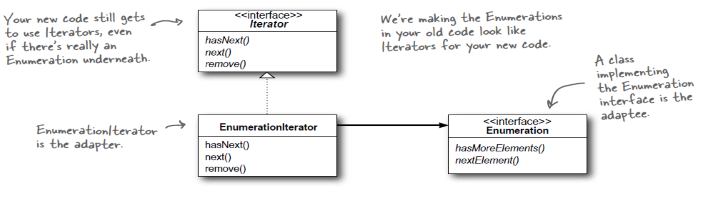
\includegraphics{GALLEYS/images/chapter6/example2}\\
\end{center}

Adapter chuyển từ hasNext(), next() sang hasMoreElements() và nextElement() là hoàn toàn có thể, nhưng vì Enumeration vốn không hỗ trợ remove() nên adapter cũng không thể làm được, không thể triển khai một hàm remove() đủ chức năng ở trong class adapter được. Lúc này, chúng ta chỉ có thể throw exception để báo cho client.